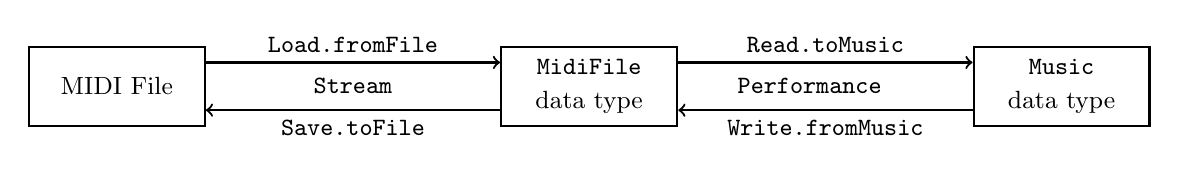
\begin{tikzpicture}[
      solid/.style={rectangle,
                    draw,
                    thick,
                    minimum height=1cm,
                    text width=2cm,
                    text badly centered},
      clear/.style={rectangle,
                    minimum height=0.5cm,
                    text width=2.5cm,
                    text badly centered}
    ]

    \draw (0,0)
          node[solid]
          (midifile)
          { \small MIDI File };
    \draw (3.0,0)
          node[clear]
          (stream)
          { \small \texttt{Stream} };
    \draw (6.0,0)
          node[solid]
          (datatype)
          { \small \texttt{MidiFile} data~type};
    \draw (8.8,0)
          node[clear]
          (performance)
          { \small \texttt{Performance} };
    \draw (12.0,0)
          node[solid]
          (musictype)
          { \small \texttt{Music} data~type};

    \draw [thick,->] (midifile.15) to 
                     node[above] { \small \texttt{Load.fromFile} }
                     (datatype.165);
    \draw [thick,<-] (midifile.-15) to
                     node[below] { \small \texttt{Save.toFile} }
                     (datatype.-165);
    \draw [thick,->] (datatype.15)  to
                     node[above] { \small \texttt{Read.toMusic} }
                     (musictype.165);
    \draw [thick,<-] (datatype.-15) to
                     node[below] { \small \texttt{Write.fromMusic} }
                     (musictype.-165);

\end{tikzpicture}
